This chapter presents the survey used for the online experiment. The database videos and the query video are included in the survey using YouTube. The online survey is powered by Google Forms, and is available online: \url{https://forms.gle/HyQAGyks2Tnj7wgc9}

\section{Title}

Content-Based Video Retrieval Experiment

\section{What is the project about?}

This dissertation project aims to create a system similar to Shazam for movies.\\

For background information, Shazam is a mobile application that allows users to match a recording to a piece of music.\\

The goal of this project is to explore how such a system could be developed to work with movies, where a user would record a screen with his phone, which will pattern match the movie to a database of movies and accurately return the movie title.

\section{Your role in this experiment}

In this experiment, you play the role of the algorithm that matches a user recording to one of the videos in the database.\\

You will be shown 6 videos from the database, followed by 1 user-recorded video.
Your goal is to mentally compare the recorded video to each video in the database to be able to rank each database video from most likely to match the recorded video to least likely.\\

When making your decision, take into account aspects of the video such as colour distribution, luminosity, textures, shapes, objects and motion, as a video matching algorithm would in real life.\\

Note: The data retrieved from this experiment will be compared to the results the of the project's matching algorithm. It will remain anonymous in locally-stored hard copies and in the final report. By submitting this form, you give consent for your data to be evaluated and used in the report. You may withdraw from the experiment at any time.

\section{Watch}

\paragraph{Database Videos}

Watch the 6 database videos that will train your ``knowledge''.

\begin{figure}[h] 
\centerline{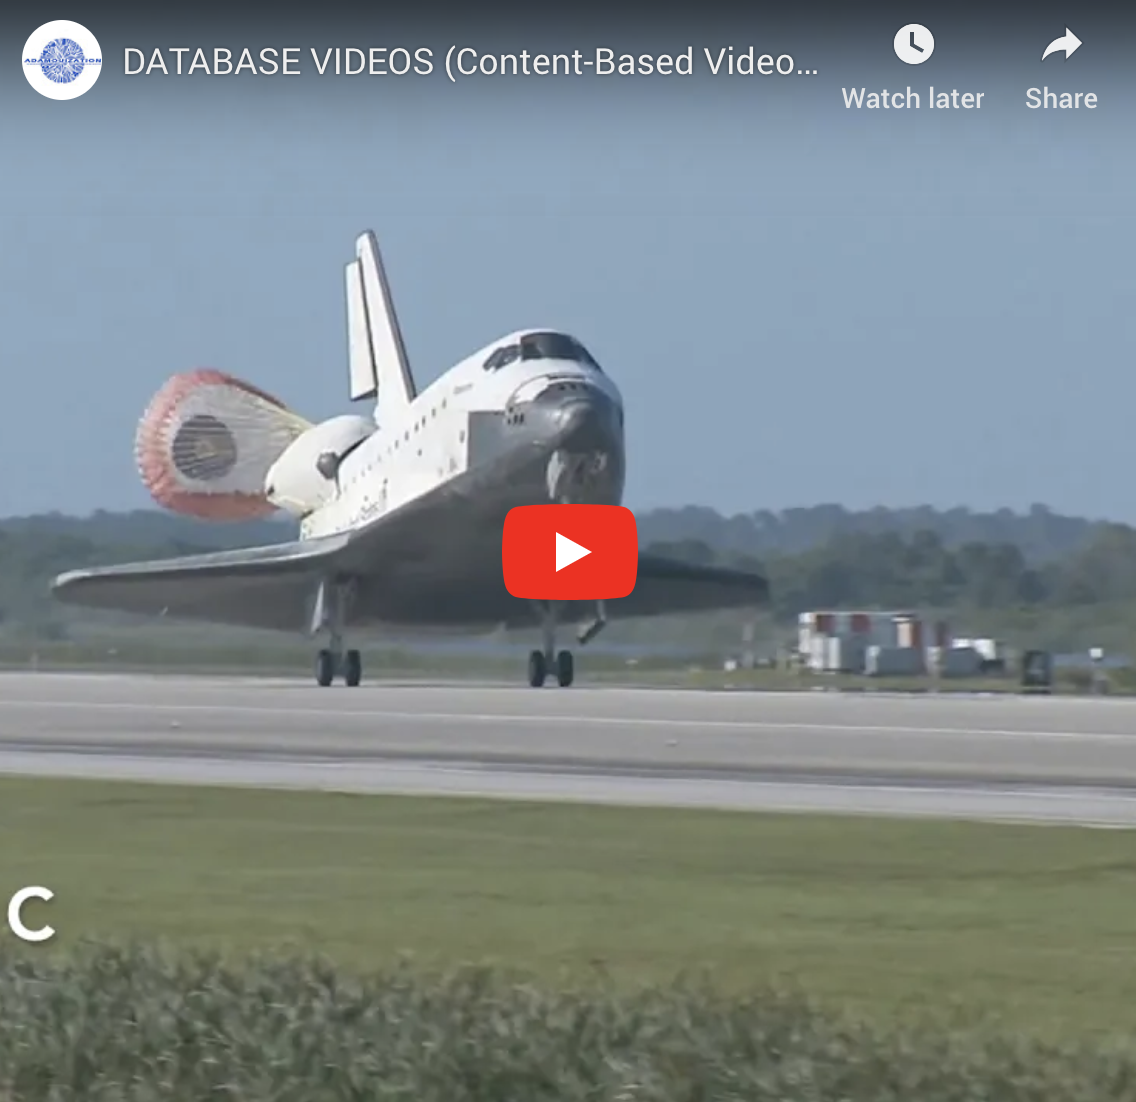
\includegraphics[width=0.50\textwidth]{figures/appendix/survey_db_videos.png}}
\caption{\label{fig:appendix-survey_db_videos}The YouTube video showing the 6 database videos used for the experiment, available online: \url{https://www.youtube.com/watch?v=BvukbK-sX9A}.}
\end{figure}

\paragraph{Query Video}

Now watch the recorded query video. Your goal is now to compare this video to the 6 previous videos you watched and to rank them based on their visual similarities.

\begin{figure}[h] 
\centerline{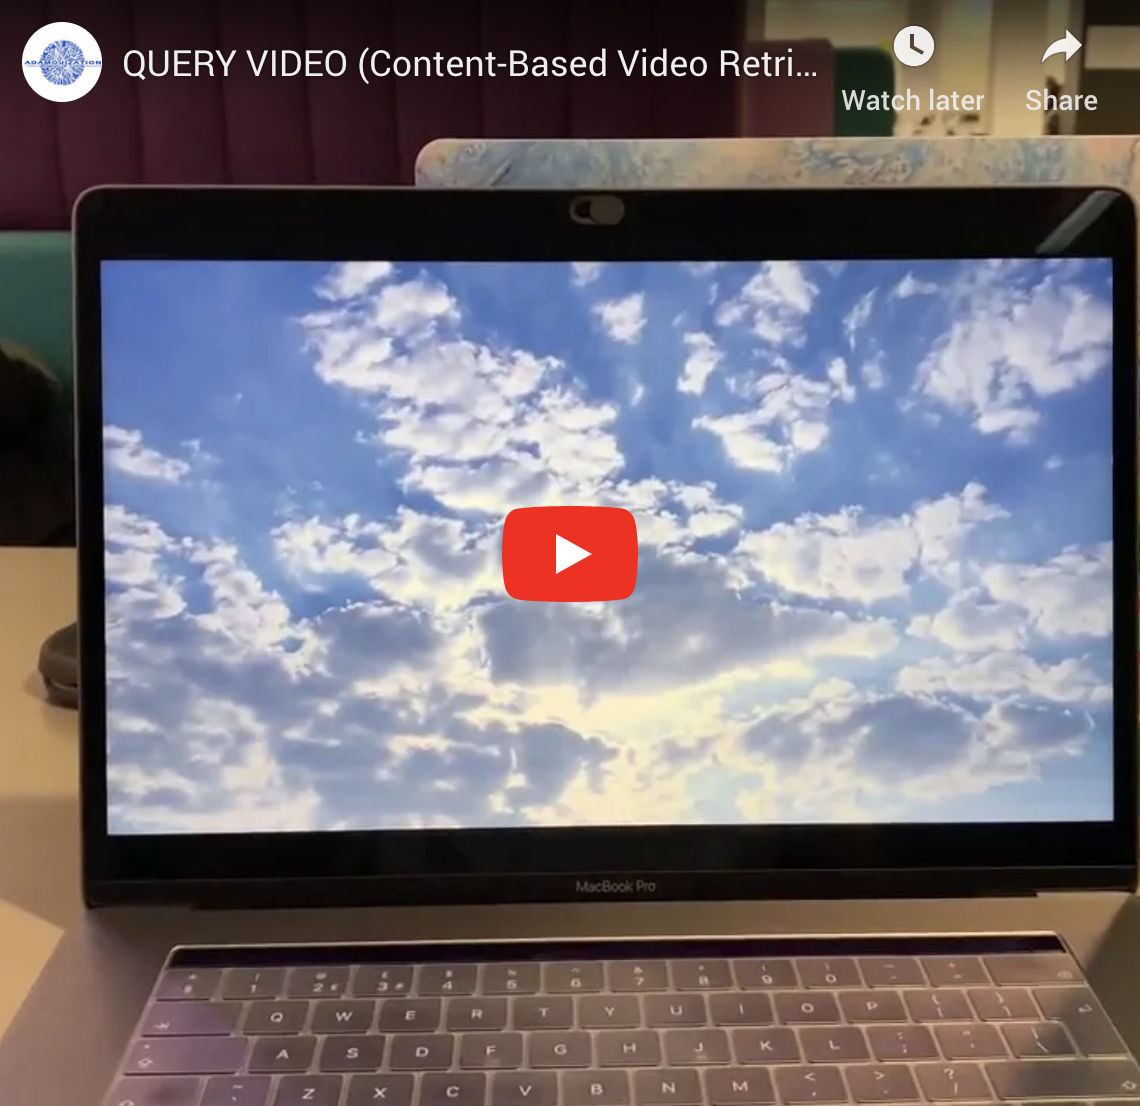
\includegraphics[width=0.5\textwidth]{figures/appendix/survey_query_video.png}}
\caption{\label{fig:appendix-survey_query_video}The YouTube video showing the query video used for the experiment, available online: \url{https://www.youtube.com/watch?v=4JPo0-aSzNE}.}
\end{figure}

\section{Rank}

\textbf{Which database video does the recorded query match the most?}\\

\begin{figure}[h] 
\centerline{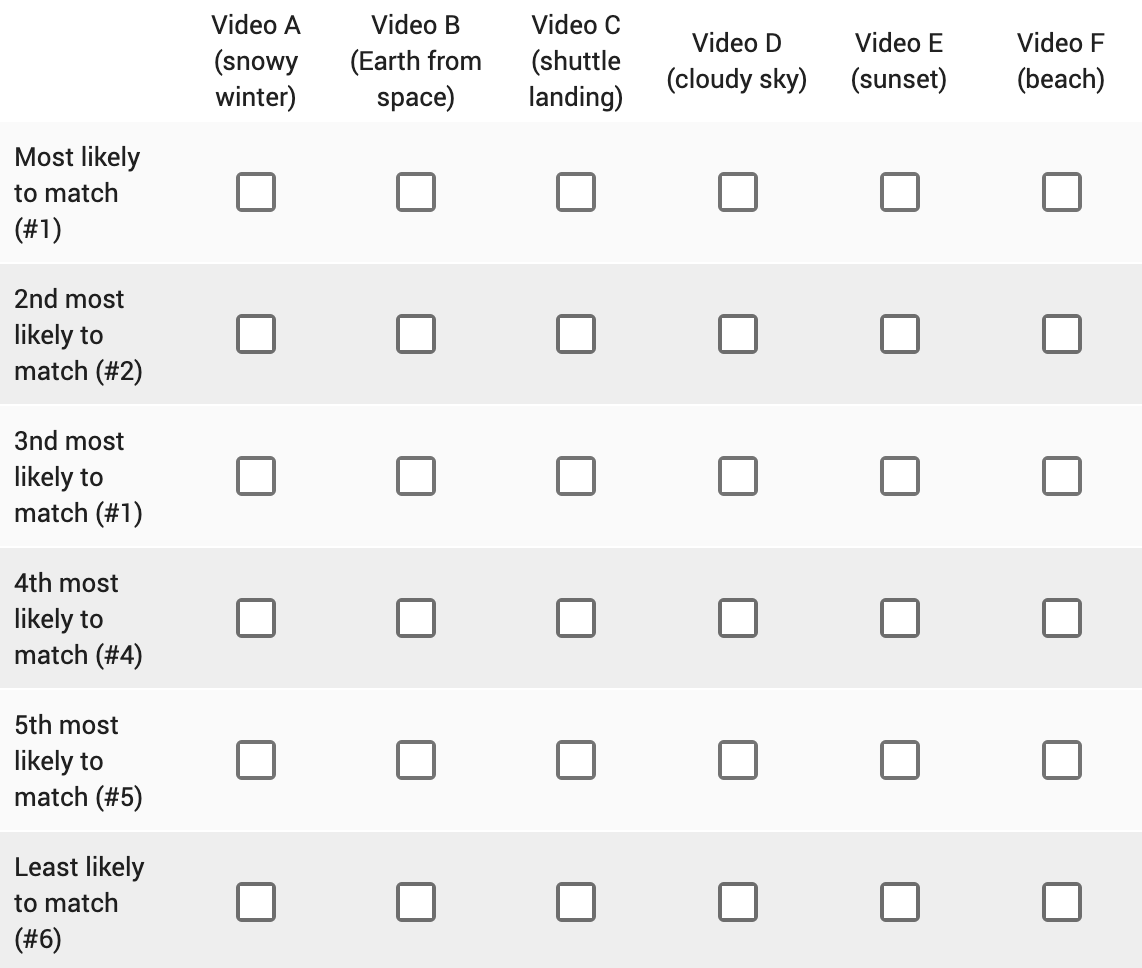
\includegraphics[width=0.55\textwidth]{figures/appendix/survey_video_ranking.png}}
\caption{\label{fig:appendix_survey_video_ranking}Screenshot of the checkbox grid used to rank the database videos from most likely to match the query video to least likely.}
\end{figure}

\textbf{Which video aspects did you consider the most when ranking them?}\\

Placeholder for long answer from participant.\\

\textbf{What do you think is the most important aspect of a video that a matching algorithm should analyse when pattern matching videos?}\\

Placeholder for short answer from participant.

\section{Confirmation Message}

(The message that is displayed to users once they have finished the experiment and submitted the Google Form).\\

\begin{quote}
    Your response has been recorded.\\

    Thank you taking part in this experiment!\\
    
    Here are my algorithm's results for comparison: 
    \begin{enumerate}
        \item cloudy-sky (video D)
        \item winter (video A)
        \item earth (video B)
        \item shuttle-landing (video C)
        \item beach (video F)
        \item sunset (video E)
    \end{enumerate}
    
    Contact details:
    \begin{itemize}
        \item Adam Jaamour: \textit{aj645@bath.ac.uk}
        \item Dr. Yong-Liang Yang (project supervisor): \textit{Y.Yang2@bath.ac.uk}
    \end{itemize}
\end{quote}